\section{April 28}
Last time, we concluded our discussion of 4-vectors by visually seeing how they transform under a Lorentz
transformation. Just like how rotational invariance requires that our vector traces out a circle, the
invariance of the spacetime interval requires that our vector travels along a hyperbola. When boosting in
multiple dimensions, we move along a \textit{hyperboloid} -- a surface created by rotating about the \( ct \)
axis. For time-like events, there is also a corresponding hyperbola:
\begin{center}
	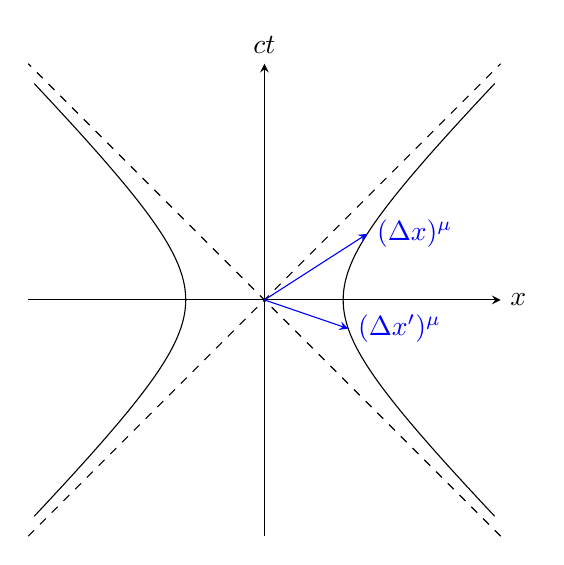
\begin{tikzpicture}
		\draw[-stealth] (-3, 0) -- (3, 0) node[right] {\( x \)};
		\draw[-stealth] (0, -3) -- (0, 3) node[above] {\( ct \)};
		\draw[dashed] (-3, -3 ) -- (3, 3);
		\draw[dashed] (3, -3) -- (-3, 3);
		\draw plot [variable = \t, samples=1000, domain=-70:70] 
			({1 / cos( \t )}, {1 * tan( \t )});
		\draw plot [variable = \t, samples=1000, domain=-70:70] 
			({-1 / cos( \t )}, {1 * tan( \t )});
		\draw[-stealth, blue] (0, 0) -- ({1 / cos(40)}, {1 * tan(40)})
			node[right] {\( (\Delta x)^{\mu} \)};
		\draw[-stealth, blue] (0, 0) -- ({1 / cos(-20)}, {1 * tan(-20)})
			node[right] {\( (\Delta x')^{\mu} \)};
	\end{tikzpicture}
\end{center}
Here, you can see that the hyperboloid is connected, so events can be Lorentz transformed into the past.  
This implies that for space-like events, there is no well defined causal structure. On the other hand, 
time-like events lie on a hyperboloid that is divided, so we do have a causal structure for time-like events. 

The transformations described up until now are denoted as \textit{active transformations}. They are
transformations that move the vector itself, while keeping the coordinate system fixed. On the contrary, we
can also imagine a \textit{passive} picture, where we alter the coordinate system instead of the vector
itself. To do this, we look back at the Lorentz transformation equations:
\[
	t' = \gamma\left( t - \frac{v}{c}x \right) \quad x' = \gamma(x - vt)
\]
Now, the \( x \)-axis corresponds to \( t = 0 \), so we have \( x' = \gamma x \). Likewise, the \( y \)-axis
corresponds to \( x = 0 \) so \( t' = \gamma t \). Therefore, our new axes transform to \( \gamma x \) and \(
\gamma t\):

\begin{center}
	\begin{tikzpicture}
		\draw[-stealth] (-3, 0) -- (3, 0) node[right] {\( x \)};
		\draw[-stealth] (0, -3) -- (0, 3) node[above] {\( ct \)};
		\draw[dashed] (-3, -3 ) -- (3, 3) node[above] {\( x = ct \)};
		\draw[dashed] (3, -3) -- (-3, 3);
		\draw[-stealth, orange] (0, 0) -- (3, 1) node[right] {\( x' \)};
		\draw[-stealth, orange] (0, 0) -- (1, 3) node[above] {\( ct' \)};
		\draw[orange] (1, 0) arc [start angle = 0, end angle = 9.46*2, radius = 1] node[midway, right] {\( \phi \)};
		% consider adding grid lines 
	\end{tikzpicture}
\end{center}
The angle \( \phi \) between the original and the altered axis is the same \( \phi \) we encountered earlier:
\( \phi = \tan^{-1}(v / c) \). In the passive picture, the event doesn't shift, but our axes and coordinate system
shifts to compensate. Just like the active frame though, this transformation allows for the breaking of
simultaneity, which you can show by tracing the grid line to the axis and figure out when that event occurs
in the boosted frame.  

\subsection{Dual Vectors}
Now, we come to the formal discussion of dual vectors. Remember from earlier, we denoted the spacetime
interval as \( ds^2 = \eta_{\mu \nu} x^{\mu}x^{\nu} \), where \( \eta \) is called the \textit{metric}. Then,
when we introduced 4-vectors, we introduced an inner product on them, defining it as \( \eta_{\mu \nu
}V^{\mu}W^{\nu} \). One way to think about this inner product is as presented, where we slap an \( \eta_{\mu
\nu} \) wherever we need it. Another way we think about it is through the context of dual vectors, by reading
the notation as \( (\eta_{\mu \nu}V^{\mu}) W^{\nu} \). Here, \( \eta_{\mu \nu}V^{\mu} \) is now a new object
which we will call a \textit{dual vector}, which we will define as \( V_{\nu} \equiv \eta_{\mu \nu}V^{\mu}
\).  

Now, notice what happens when we transform a vector into a dual vector. Suppose we start with the standard
vector \( V^{\mu} = \begin{pmatrix} V^{0} & V^{1} & V^{2} & V^{3} \end{pmatrix} \), and we now consider its
dual:
\[
	V_{\mu} = \eta_{\mu \nu}V^{\nu} = \begin{pmatrix} \eta_{0 \nu}V^{\nu} & \eta_{1 \nu} V^{\nu} & \eta_{2
		\nu} V^{\nu} & \eta_{3 \nu}V^{\nu}  \end{pmatrix} = \begin{pmatrix} -V^{0} & V^{1} & V^2 & V^3 \end{pmatrix}
\]
So compared to \( V^{\mu} \), the dual \( V_{\mu} \) has its time direction reversed. This has implications
for how the dual vector transforms, since we ultimately still want the dot product to be invariant. To see
how the dual transforms, we will have to set up some machinery first. Define the inverse matrix \( \eta^{\mu
\nu} \) such that \( \eta^{\mu \nu} \eta_{\nu \rho} = \delta^{\mu}_\rho \). Ironically enough, the explicit
form of \( \eta^{\mu \nu} \) actually looks the same as \( \eta_{\mu \nu} \):
\[
	\eta^{\mu \nu} = \begin{pmatrix} -1 &  & & \\ & 1 & & \\ & & 1 & \\ && & 1 \end{pmatrix}
\]
but it should be understood as a different object entirely. 

\begin{aside}
	Now that we're dealing with upper and lower indices, now's a good time to talk about why we never really
	cared about the ordering of the indices when taking a dot product. It's because they are in fact equal:
	\[
		\eta_{\mu \nu} V^{\mu}W^{\nu} = V_{\nu}W^{\nu} = V_\nu(\eta_{\nu \rho} W_{\rho}) = V^{\rho}W_{\rho}
	\]
\end{aside}
Now, recall that \( \Lambda \) satisfies \( \eta_{\mu \nu} \Lambda^{\mu}_\rho \Lambda^{\nu}_{\sigma} =
\eta_{\rho \sigma} \). Now, we multiply on the right by \( (\Lambda^{-1})^{\sigma}_\lambda \), and simplify
it:
\begin{align*}
	\eta_{\mu \nu}\Lambda^{\mu}_{\rho}\Lambda^{\nu}_\sigma \left( \Lambda^{-1} \right)^{\sigma}_\lambda &=
	\eta_{\rho \sigma}\left( \Lambda^{-1} \right)^{\sigma}_\lambda\\
	\eta_{\mu \nu}\Lambda^{\mu}_\rho \delta^{\nu}_\lambda &= \eta_{\rho \sigma}
	\left(\Lambda^{-1}\right)^{\sigma}_\lambda\\
	\eta_{\mu \lambda} \Lambda^{\mu}_\rho &= \eta_{\rho \sigma}\left( \Lambda^{-1} \right)^{\sigma}_\lambda 
\end{align*}
Now, we \textit{define} \( \Lambda_{\lambda \rho} \equiv \eta_{\mu \lambda}\Lambda^{\mu}_\rho \), which gives
us the relation:
\begin{equation}
	\Lambda_{\lambda \rho} = \left( \Lambda^{-1} \right)_{\rho \lambda}
\end{equation}
This equation can roughly be interpreted as saying that the inverse of \( \Lambda \) is its transpose. Now
with \( \Lambda^{-1} \) introduced, how does \( V_{\mu} \) transform under a Lorentz transformation? 
\begin{align*}
	V'_{\mu} = \eta_{\mu \nu}V'^{\nu} &= \eta_{\mu \nu} \Lambda^{\nu}_\rho V^{\rho}\\
	&= \Lambda_{\mu \rho}V^{\rho} \\ 
	&= \left( \Lambda^{-1} \right)_{\rho \nu} V^{\rho} \\ 
	&= \left( \Lambda^{-1} \right)^{\rho}_\nu V_\rho
\end{align*}
So in contrast with \( V^{\mu} \), the dual \( V_{\mu} \) uses the inverse \( \Lambda^{-1} \) to transform.
This way, the dot product:
\begin{align*}
	V^{\mu}W_{\mu} \to V'^{\mu}W'_{\mu} &= \left( \Lambda^{\mu}_\rho V^{\rho} \right)\left( \left(
	\Lambda^{-1} \right)^{\lambda}_\mu W_\lambda \right)\\
	&= \left( \Lambda^{-1} \right)^{\lambda}_\mu \Lambda^{\mu}_\rho V^{\rho}W_\lambda \\ 
	&= \delta^{\lambda}_\rho V^{\rho}W_\lambda \\ 
	&= V^{\lambda}W_\lambda 
\end{align*}
Hence the invariance of the dot product is preserved.  
 

 






